\documentclass[11pt, letterpaper]{article}
\usepackage[T1]{fontenc}
\usepackage[utf8]{inputenc}
\usepackage[includehead, margin=0.75in]{geometry}
\usepackage{fancyhdr}
\usepackage[british]{babel}
\usepackage{esvect}
\usepackage{amsmath}
\usepackage{amsthm}
\usepackage{amssymb}
\usepackage{amstext}
\usepackage{soul}
\usepackage{color}
\usepackage{colortbl}
\usepackage{graphicx}
\usepackage{siunitx}
\usepackage{textgreek}
\usepackage{xspace}
\usepackage{lastpage}
\usepackage{lipsum}
\definecolor{error}{rgb}{255,255,0}
\newcommand{\degree}{\ensuremath{{}^{\circ}}\xspace}

\begin{document}

\fancypagestyle{plain}{%
\fancyhf{}%
\fancyhead[L]{PHYS 211L \\ Dr.\@ Streider}
\fancyhead[R]{H. Ryott Glayzer \\ \today}%
\fancyhead[C]{Prelab \\ \textit{Introduction to Motion Detectors}}%
\fancyfoot[L]{\textsc{Prelab Report No. 1}}%
\fancyfoot[C]{\thepage~of~\pageref{LastPage}}
\fancyfoot[R]{\textsc{University Physics I Lab}}
}


\title{Prelab No. 1}
\author{H. Ryott Glayzer}
\date{\today}


\maketitle



\section{Particle Motion given by $x(t) = 7.8 + 9.2t - 2.1t^{3}$}
\subsection{Instantaneous velocity}
The instantaneous velocity of the particle can be determined by the first derivative
of the equation of motion. 
The motion of the particle is defined as the relation
\begin{equation}
	x(t) = 7.8 + 9.2t - 2.1t^{3},
\end{equation}
the derivative of which can be found via the power rule:
\begin{equation}
	\dot{x}(t) = 9.2 - 6.3t^{2}.
\end{equation}
The instantaneous velocity given by $\dot{x}(t)$ is time-dependent, as the velocity
is not constant over time.

\subsection{Zero Velocity}
The velocity of the particle can be found via
\begin{equation}
	\dot{x}(t)=9.2-6.3t^{2}.
\end{equation}
The zero of this function that lies in the positive-time domain represents a
velocity of zero.
Thus, the time where $\dot{x}(t) = 0$ can be found by setting the function
equal to zero and solving for $t$:
\begin{equation}
\begin{align}
	0 &= 9.2-6.3t^{2}\\
	9.2 &= 6.3t^{2}\\
	\frac{92}{63} &= t^{2}\\
	t &= \frac{2}{3}\sqrt{\frac{23}{7}}\\
	t &\approx 1.2
\end{align}
\end{equation}

\subsection{Instantaneous Acceleration}

The instantaneous acceleration of the particle can be found via the second 
derivative of the equation of motion, or

\begin{equation}
	\ddot{x} = -12.6t.
\end{equation}

This acceleration is time dependent, and takes jerk into account. 

\subsection{Zero acceleration}

The particle has zero acceleration at the time $t=0$.


\section{Particle Motion given by displacement.}

\subsection{Constant Velocity by Kinematics}
Given $\Delta x_{1 s} = 14$ and $\Delta x_{2s} = 42$, as well as the assumption of a 
constant velocity, we can take 
\begin{equation}
	\vv{v} = \frac{\vv{\Delta x}}{\Delta t}
\end{equation}
and input the values 
\begin{equation}
	\vv{v} = \frac{42-14 \;m}{2-1 \;s}
\end{equation}
to find 
\begin{equation}
	\vv{v} = 28 \;m/s
\end{equation}

\subsection{Plotting the data}
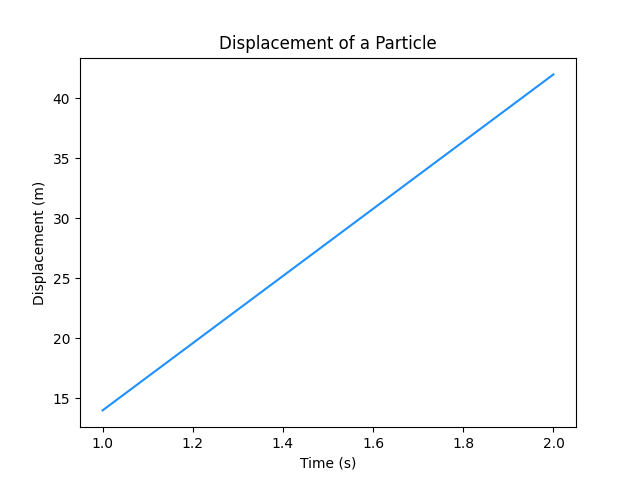
\includegraphics{plot_2a.png}

This plot does reflect my earlier predictions.














\end{document}





%%%%%%%%%%%%%%%%%%%%%%%%%%%%%%%%%%%%%%%%%%%%%%%%%%%%%%%%%%%%%%%%%%%%%%%%%%%%%%%
%%%                                 Copypasta                               %%%
%%%%%%%%%%%%%%%%%%%%%%%%%%%%%%%%%%%%%%%%%%%%%%%%%%%%%%%%%%%%%%%%%%%%%%%%%%%%%%%

% Table for questions with multiple parts

% \begin{center}
% 	\begin{tabular}{|c|c|c|c|c|}
% 		\hline
% 		_ & _ & _ & _ & _ \\
% 		\hline
% 		_ & _ & _ & _ & _ \\
% 		\hline
% 	\end{tabular}
% \end{center}
